\documentclass{article}

% Language setting
\usepackage[english]{babel}

% Set page size and margins
% `a4paper' for EU standard size
\usepackage[a4paper,top=2cm,bottom=2cm,left=3cm,right=3cm,marginparwidth=1.75cm]{geometry}

% Load packages
\usepackage{amsmath}
\usepackage{graphicx}
% \usepackage[colorlinks=true, allcolors=blue]{hyperref}

\begin{document}

\begin{titlepage}
    \begin{center}
        \vspace*{1cm}

        \huge{Akademia Górniczo-Hutnicza}\\
        \large{im. Stanisława Staszica w Krakowie}

        \vspace{0.5cm}

        \large{Wydział Informatyki, Elektroniki i Telekomunikacji}

        \vspace{0.5cm}

        \large{Instytut Informatyki}

        \vspace{1cm}

        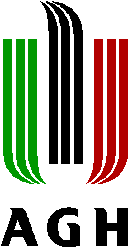
\includegraphics{img/agh.png}

        \vspace{1cm}

        \large\textsc{STUDIA PODYPLOMOWE
        \\ANALIZA DANYCH – DATA SCIENCE}

        \vspace{1cm}
        \large{Projekt dyplomowy}

        \vspace{0.8cm}

        \textbf{Analysis of Prediction Power of Information about Payment Delay to Forecast Financial Problems}

        \vspace{1.5cm}

        \textbf{Autor}\\
        \textbf{mgr inż. Konrad J. Gródek}

        \vspace{0.8cm}
        \textbf{Opiekun Projektu}\\
        \textbf{dr inż. Robert Marcjan}


        \vfill

        \large{Kraków, 2023}

        \end{center}
    \end{titlepage}

\pagebreak


\begin{abstract}
\vspace{1cm}

The project will focus on information about bill payment experiences - information coming from various
sources, from companies that report the bill issue and payment day. The bill may be paid with certain
delay or ahead of time. In the latter case the term “delay” makes no lexical sense, but in order to keep consistent naming, the difference in days between issue and payment will be hereinafter referred to as delay, which may take negative value to picture the bill being paid in advance.\par
The first step will be to assess the quality of the sources and to choose those, where the information is reliable and have potential for further analysis. It will include providing distribution of the data
respecting sociodemographic attributes to determine the typical profile of an average customer. The
goal of the second part is to find statistically proved connections between the pay-delay details and the
financial issues that had happened afterwards. The details of the payment will cover attributes like the
delay in days, the amount and the industry of bill issuer. It is important to explore also the tendencies
that occur for these numbers over time. The analysis must also take into consideration the gradual
nature of the “financial problems”, which take one of few severity levels, from collection notice to
bankruptcy.\par
The analysis will be performed on data collected by Crif AG from Zurich, leading economic information
bureau in Switzerland. The data, neither of the bill issuer nor bill payer, must not be revealed in the final
project documentation.

\end{abstract}

\pagebreak

\tableofcontents

\pagebreak

\section{Introduction}

This section will provide more elaborate description of the problem and will provide more information on the data, which will be used in the project.

\subsection{The problem}

Crif AG is a Swiss economic information bureau delivering solutions for clients interested in checking creditworthiness of both private and corporate individuals. For number of years the company was collecting information about paid bills issued by Crif's customers. Till now the information was not included in the procedures of calculating probability of default (so-called \textit{scoring}). The aim of this work is to explore the potential hidden in the data to support process of evaluating creditworthiness. In order to do that, certain attributes of the data must be explored and confronted with history of negative payment information (debts). As a result, statistical evidence will prove - or not - existence of correlation between those attributes (variables) and the probability of default. The correlation must be backed up by plausible causation.\par
It is important to stress that the analysis will be performed exclusively on data recorded for private persons. \textbf{TBD: how about single-person-companies?}\par

\subsection{The data}

The data in scope of the analysis can be divided into three types: payment delay, debt and legal entity information.

\subsubsection{Payment delay}

As it was already mentioned, the \textbf{payment delay} term may be misleading. What is understood by this term can be more precisely explained as \textbf{the performance of paying the bill}. Once issued, the bill may be paid in advance, on time or with a certain delay.\par
\vspace{5pt}
The \textbf{payment delay} comes with the following attributes:
\begin{itemize}
    \item Bill issue date
    \item The delay measured as the number of days between the issue and payment dates. May be negative.
    \item The identification of the bill issuer (\textit{source})
    \item The industrial sector of the bill issuer
    \item The identification of the bill payer
\end{itemize}

Most of listed attributes are obligatorily present in the data set. The exception is the industrial sector of the bill issuer, which may be unknown.

\subsubsection{Debt}

The \textbf{debt} is a recorded negative payment experience. It has certain severity and validity period. The list of attributes:
\begin{itemize}
    \item Validity period: start and end date (note that the later can be in future)
    \item Amount owned - will not be used in the analysis
    \item Severity
    \item The identification of the debtor
\end{itemize}

All listed attributes are obligatorily present in the data set.

\subsubsection{Legal entity}

Only sociodemographic information is accessible for sake of this analysis. This includes only very limited set of attributes:

\begin{itemize}
    \item Age (rounded to full years)
    \item Gender
    \item Location (the highest accuracy: city/town/village)
\end{itemize}

Each of the listed attributes may appear undefined (none of them is obligatory).


\subsection{The quality challenge}
One of the challenges to be faced in order to answer on the formulated problem is how to deal with the source quality issues. The data is coming from various sources and the quality of delivery is often questionable. The part of the analysis will be to measure the quality of the sources, maybe to categorize them in quality groups.\par
How to categorize the sources? What measurements shall be used to calculate the quality of the source? The following ideas will be explored:
\begin{itemize}
    \item \textbf{Number of recorded payments}. The simplest - but often misleading - way to asses the usefulness of the data source. Obviously, the more records the better, but if the data is not reliable, the large volume will not make it better.
    \item \textbf{Average number of paid bills per person}. From the two sources the one providing longer history of payments per person will most likely be more useful than the one providing single payments.
    \item \textbf{Ratio of missing values and outliers.} Surely high ratio of the data, which remain undefined (applies mostly to sociodemographic attributes) makes the source less attractive. The same applies to source with high number of unreliable data
    \item \textbf{Overrepresentation of "0-delay" records}. If the source reports that the bills are paid exactly on time by vast majority of payers, its predictive power will be close to zero.
    \item \textbf{Data continuity versus clustered information}. Partly related to the above. There is nothing bad if the source reports the delay in certain periods (e.g. every week or month), but in such a case the source may be treated differently from the one that reports in more continuous manner.
    \item \textbf{Variability}. Except continuity, a desired situation is to have more variable data, spanning over longer periods, including high and low amounts, scrupulous payers as well as those neglecting liabilities.
\end{itemize}

\pagebreak

\section{Exploratory analysis}

\subsection{The data overview}

Here I will present the overview on the whole set of data

\subsection{Analysis of sources}

In this section results of analysis of differences and similarities of the sources will be presented. The goal is to find a way (or prove it is impossible) to categorize the sources from quality point of view

\subsubsection{Overview}

In here the overview on data from perspective of single source will be presented.

\subsubsection{Chosen sources analysis - preliminary}
\textbf{Note: this is preliminary analysis, most likely will not be part of final document}.\par

In this section three example sources will be checked in details. The names of the sets (\textit{Aarau, Baar, Cham}) does not correspond to any characteristic of the sources. These are just nicknames, taken from small Swiss towns\par
\vspace{10pt}
\textbf{Basic counts}\par
Table \ref{tab:chosen-sources-quantitative} presents the comparison between the three sets respecting the counts of the records and average delay.\par

\begin{table}[!htbp] \centering
  \caption{Quantitative overview of the chosen sources}
  \label{tab:chosen-sources-quantitative}
\begin{tabular}{@{\extracolsep{5pt}} cccc}
\\[-1.8ex]\hline
\hline \\[-1.8ex]
 & Bills count & Persons count & Avg bills per person \\
\hline \\[-1.8ex]
Aarau & $3,913,966$ & $1,492,493$ & $2$ \\
Baar & $8,361,151$ & $1,128,751$ & $7$ \\
Cham & $3,311,629$ & $145,421$ & $22$ \\
\hline \\[-1.8ex]
\end{tabular}
\end{table}

First noticeable difference is how many on average payment delays are delivered per person. Clearly \textit{Aarau} delivers only single entries, but for large number of different legal entities, whereas in \textit{Cham} we can expect more payment delays per person.\par

\vspace{10pt}

\textbf{Identify outliers}\par

Table \ref{tab:outlier-def} presents definition of unreliable data (outliers)

\begin{table}[!htbp]
    \centering
    \caption{Rules to identify outliers}
    \label{tab:outlier-def}
    \begin{tabular}{c c p{0.6\linewidth}}
    \hline\hline \\
    Attribute & Value & Reasoning \\
    \hline \\
    Minimum delay & -30 & Usually the bill should be paid after a month, so if one pays it immediately, the delay is -30 \\
    Maximum delay & 182 & An arbitrary number. The assumption is that delay greater than half a year should trigger collection of the overdue, which makes it being a \textit{debt}, no longer a \textit{delay} \\
    Minimum amount & 1 CHF & Pretty obvious, the smaller amounts are considered to be incorrect \\
    Maximum amount & 10000 CHF & An arbitrary number chosen by examining the data \\
    \end{tabular}
\end{table}

Once defined, the outliers in each of the sources can be counted. Table \ref{tab:outliers-ratio} presents the results.\par

\begin{table}[hbt!] \centering
  \caption{Ratio of outliers}
  \label{tab:outliers-ratio}
\begin{tabular}{@{\extracolsep{5pt}} cccc}
\\[-1.8ex]\hline
\hline \\[-1.8ex]
 & Incorrect delay & Incorrect amount & To reject \\
\hline \\[-1.8ex]
Aarau & $8.770$ & $0.005$ & $8.773$ \\
Baar & $0.285$ & $0.135$ & $0.419$ \\
Cham & $0.742$ & $0.057$ & $0.793$ \\
\hline \\[-1.8ex]
\end{tabular}
\end{table}

The high number of outliers in case of \textit{Aarau} is disturbing (out of scope right now).\par

\vspace{10pt}

\textbf{Comparison of descriptive statistics}

Tables \ref{tab:src-summary-aarau}, \ref{tab:src-summary-baar}, \ref{tab:src-summary-cham} present the summary statistics of the three chosen sets.

\begin{table}[!htbp] \centering
  \caption{Summary of Aarau data set}
  \label{tab:src-summary-aarau}
\begin{tabular}{@{\extracolsep{5pt}}lccccc}
\\[-1.8ex]\hline
\hline \\[-1.8ex]
Statistic & \multicolumn{1}{c}{N} & \multicolumn{1}{c}{Mean} & \multicolumn{1}{c}{St. Dev.} & \multicolumn{1}{c}{Min} & \multicolumn{1}{c}{Max} \\
\hline \\[-1.8ex]
delay\_days & 3,570,582 & 6.787 & 34.483 & $-$30 & 182 \\
invoiced\_amount & 3,570,582 & 235.372 & 390.469 & 1.000 & 10,000.000 \\
sex & 3,566,986 & 1.635 & 0.481 & 1 & 2 \\
age & 3,545,847 & 41.968 & 14.222 & 18 & 100 \\
\hline \\[-1.8ex]
\end{tabular}
\end{table}

\begin{table}[!htbp] \centering
  \caption{Summary of Baar data set}
  \label{tab:src-summary-baar}
\begin{tabular}{@{\extracolsep{5pt}}lccccc}
\\[-1.8ex]\hline
\hline \\[-1.8ex]
Statistic & \multicolumn{1}{c}{N} & \multicolumn{1}{c}{Mean} & \multicolumn{1}{c}{St. Dev.} & \multicolumn{1}{c}{Min} & \multicolumn{1}{c}{Max} \\
\hline \\[-1.8ex]
delay\_days & 8,326,089 & $-$0.847 & 22.901 & $-$30 & 182 \\
invoiced\_amount & 8,326,089 & 34.731 & 38.331 & 1.000 & 9,765.000 \\
sex & 8,323,436 & 1.819 & 0.385 & 1 & 2 \\
age & 8,187,482 & 49.164 & 14.630 & 18 & 100 \\
\hline \\[-1.8ex]
\end{tabular}
\end{table}

\begin{table}[!htbp] \centering
  \caption{Summary of Cham data set}
  \label{tab:src-summary-cham}
\begin{tabular}{@{\extracolsep{5pt}}lccccc}
\\[-1.8ex]\hline
\hline \\[-1.8ex]
Statistic & \multicolumn{1}{c}{N} & \multicolumn{1}{c}{Mean} & \multicolumn{1}{c}{St. Dev.} & \multicolumn{1}{c}{Min} & \multicolumn{1}{c}{Max} \\
\hline \\[-1.8ex]
delay\_days & 8,326,089 & $-$0.847 & 22.901 & $-$30 & 182 \\
invoiced\_amount & 8,326,089 & 34.731 & 38.331 & 1.000 & 9,765.000 \\
sex & 8,323,436 & 1.819 & 0.385 & 1 & 2 \\
age & 8,187,482 & 49.164 & 14.630 & 18 & 100 \\
\hline \\[-1.8ex]
\end{tabular}
\end{table}

\vspace{20pt}

\textbf{Correlation and histograms}\par

In the next step the analysis of correlation between delay, amount and age will be performed. The analysis was made on 10k random subset of data.\par
Figures \ref{fig:ex-src-aarau-corr}, \ref{fig:ex-src-baar-corr} and \ref{fig:ex-src-cham-corr} shows the results. Clearly there are no correlations between the listed attributes, which actually is a good sign.

\begin{figure}
    \centering
    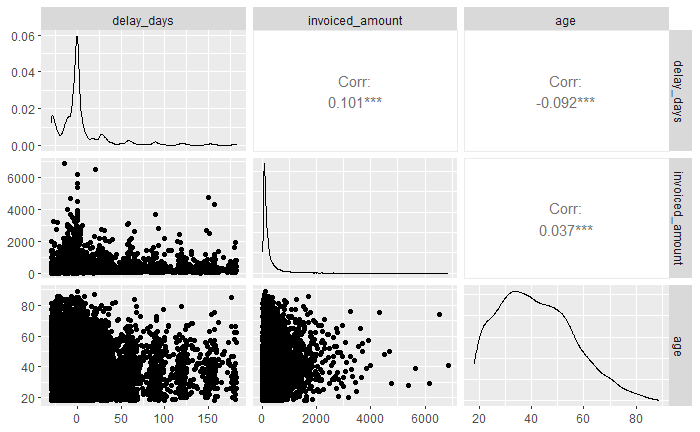
\includegraphics[width=\textwidth]{fig/ex-src-aarau-corr.png}
    \caption{Correlation analysis for Aaarau data set}
    \label{fig:ex-src-aarau-corr}
\end{figure}
\begin{figure}
    \centering
    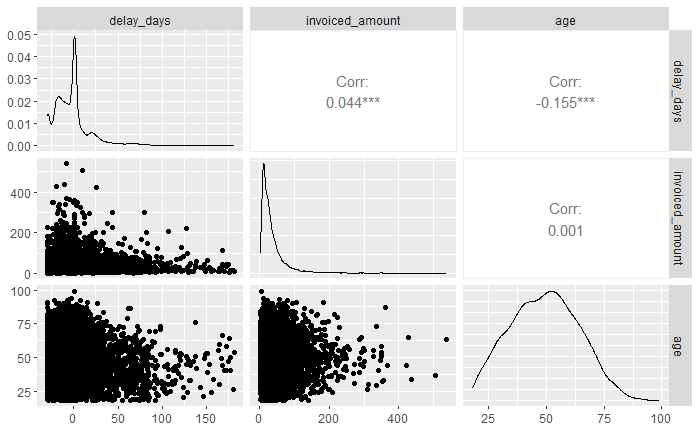
\includegraphics[width=\textwidth]{fig/ex-src-baar-corr.png}
    \caption{Correlation analysis for Baar data set}
    \label{fig:ex-src-baar-corr}
\end{figure}
\begin{figure}
    \centering
    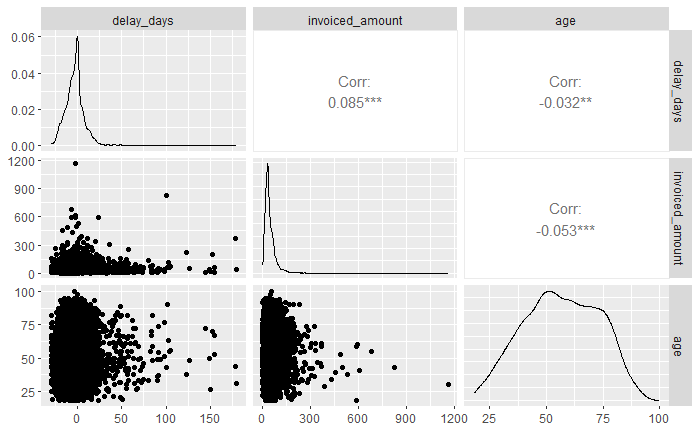
\includegraphics[width=\textwidth]{fig/ex-src-cham-corr.png}
    \caption{Correlation analysis for Cham data set}
    \label{fig:ex-src-cham-corr}
\end{figure}

\subsubsection{The typical payer}

Subsequent sources may differ not only in quality, but also in typical payer of their bills. For example: overrepresentation of women, more elderly payers, higher amounts. \textbf{Idea: to present sources on two-dimensions: average amount versus average delay. }

\subsection{The source quality}

\subsubsection{Proposed categorization / quality measurement}

\subsubsection{The results}

\pagebreak

\section{Prediction analysis}

The main part of the project. The following hypothesis will be verified (provisional list):
\begin{itemize}
    \item Average delay versus probability of default
    \item Growing or decreasing \textbf{overdue} amount of average bill over time versus probability of default
    \item The payment delay tendency over time versus probability of default
\end{itemize}

\pagebreak

\section{Conclusions}

Are there statistically proven relations between payment delay history and the later new debts arrival?
Is this connection reliable? Can it be told as a plausible story? Is it dependent on the quality class of the source? If more than one relation is identified, explain which is better, describe the difference (in numbers as well as in words)

\end{document}